
\chapter{Resultados e Discussões}
%%%%%%%%%%%%%%%%%ALTERADO%%% %%%%%%%%%%%%%%%%%%%%
\label{cap:resultados}
 Neste capítulo são apresentados os resultados obtidos após o desenvolvimento do protótipo e a análise dessas informações. O desenvolvimento deste projeto cumpriu as etapas planejadas e teve como resultado um protótipo com dois perfis: O perfil catador, o qual é responsável pelo recolhimento do material e o perfil separador, que solicita o serviço da coleta de resíduos sólidos.

Para avaliar a usabilidade da aplicação, foram realizados testes com 4 pessoas, onde estas responderam um questionário com perguntas avaliativas. O roteiro da avaliação pode ser visualizado no ANEXO A. No questionário foram realizadas sete perguntas com notas de um a cinco. Durante a avaliação foi possível observar a utilização do protótipo pelos participantes e os pontos que poderiam ser melhorados, a fim de facilitar o uso da aplicação.

No final do testes foi coletado o questionário de avaliação dos participantes com os itens avaliados, sendo estas informações representadas na \autoref{fig:resultados}.

\begin{figure}[H]
	\begin{Center}
		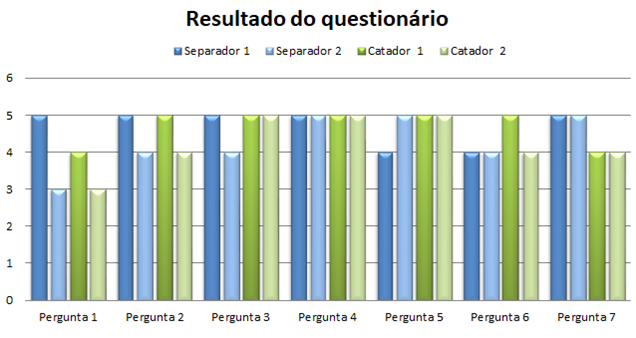
\includegraphics[width=5.0in,height=3.06in]{./media/resultados.png}
	\end{Center}
\caption{Gráfico dos resultados obtidos do questionário}
\label{fig:resultados}
\end{figure}

Na \autoref{fig:resultados} citada acima foi possível observar que foram criados quatro perfis de usuário: dois perfis separadores e dois perfis catadores. A média dos resultados das perguntas foi satisfatória.

O \autoref{cod:cadbanc0} é responsável por salvar o usuário catador no \textit{firebase realtime database}. A linha 3 do \autoref{cod:cadbanc0}, consiste na criação do nó (\textit{child}) denominado “Catadores”, onde cada catador possui um identificador (\textit{id}), onde seus dados são salvos (\textit{setValue}).

\begin{codigo}[H]
\begin{lstlisting}[language=Java]
public void salvar(){
    DatabaseReference databaseReference = ConfiguracaoFirebase.getFirebase();
    databaseReference.child("Catadores").child(getId()).setValue(this);
}
\end{lstlisting}
\caption{Salvar usuário catador no banco de dados}
\label{cod:cadbanc0}
\end{codigo}


Na \autoref{fig:login} a seguir, é apresentada a tela inicial da aplicação. 
%%%%%%%%%%%%%%%%%%%% Figure/Image No: 54 starts here %%%%%%%%%%%%%%%%%%%%

\begin{figure}[H]
	\begin{Center}
		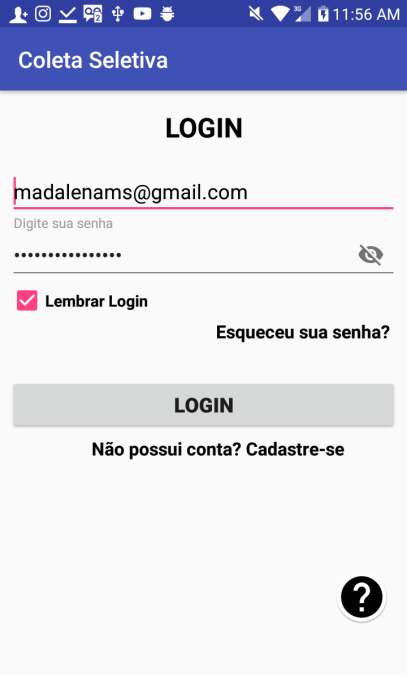
\includegraphics[width=1.85in,height=2.94in]{./media/image34.png}
	\end{Center}
\caption{Tela de Login}
\label{fig:login}
\end{figure}
%%%%%%%%%%%%%%%%%%%% Figure/Image No: 54 Ends here %%%%%%%%%%%%%%%%%%%%
Na tela inicial (\autoref{fig:login}) da aplicação citada acima, o usuário já cadastrado irá informar seu \textit{e-mail} e senha e realizar o \textit{login} no sistema. A aplicação permite a visualização da senha digitada e o armazenamento dos dados de autenticação. Caso o usuário tenha esquecido seu \textit{e-mail} e/ou senha, poderá recuperá-lo em “Esqueceu sua senha?”. Caso não possua cadastro, o usuário irá clicar em “Não possui conta? Cadastre-se”, e será redirecionado para a tela de cadastro. No caso de dúvidas referentes à definição dos perfis, basta o usuário clicar no ícone de interrogação.

Na \autoref{fig:cadcatador} a seguir, é apresentado o processo de cadastro do usuário catador.

%%%%%%%%%%%%%%%%%%%% Figure/Image No: 44 starts here %%%%%%%%%%%%%%%%%%%%

\begin{figure}[H]
	\begin{Center}
		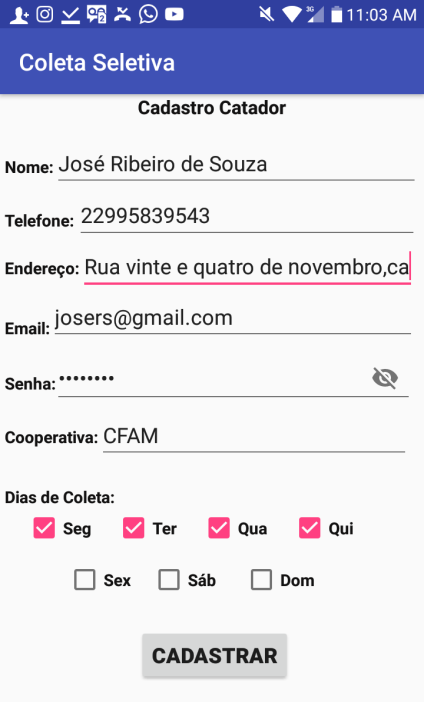
\includegraphics[width=1.92in,height=3.06in]{./media/image5.png}
	\end{Center}
\caption{Cadastro do usuário catador}
\label{fig:cadcatador}
\end{figure}

%%%%%%%%%%%%%%%%%%%% Figure/Image No: 44 Ends here %%%%%%%%%%%%%%%%%%%%

A \autoref{fig:cadcatador} citada acima, apresenta a tela de cadastro do usuário catador, onde o mesmo irá informar o nome, o telefone, o endereço, o \textit{e-mail}, a senha, a cooperativa associada e os dias que realiza a coleta. Após o preenchimento de todos esses dados, o usuário irá clicar no botão "cadastrar" e será exibido na tela a confirmação do cadastro. Se algum dado não for preenchido ou \textit{e-mail} já tenha sido cadastrado, a aplicação irá informá-lo.

Na \autoref{fig:cadseparador} abaixo, é apresentado o processo de cadastro do usuário separador. 
%%%%%%%%%%%%%%%%%%%% Figure/Image No: 45 starts here %%%%%%%%%%%%%%%%%%%%

\begin{figure}[H]
	\begin{Center}
		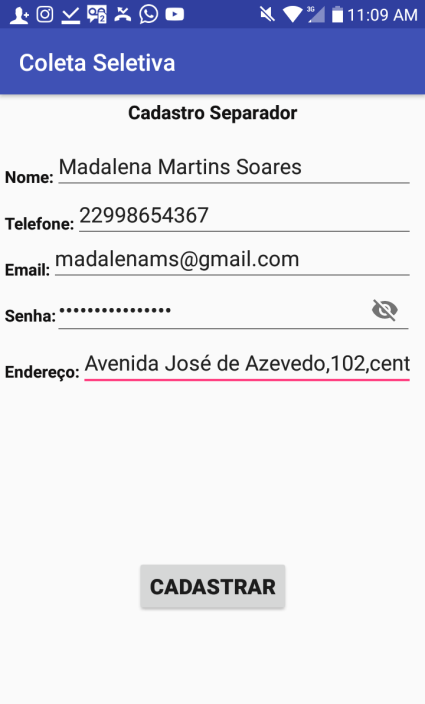
\includegraphics[width=1.93in,height=3.06in]{./media/image3.png}
	\end{Center}
	\caption{Cadastro do usuário separador}
	\label{fig:cadseparador}
\end{figure}

A \autoref{fig:cadseparador} citada acima, apresenta a tela de cadastro do usuário separador, onde o mesmo irá informar o nome, o telefone, o \textit{e-mail}, a senha e o endereço. Após o preenchimento de todos esses dados, o usuário irá clicar no botão "cadastrar" e será exibido na tela a confirmação do cadastro. Se algum dado não for preenchido ou \textit{e-mail} já tenha sido cadastrado, a aplicação irá informá-lo.


Na \autoref{fig:listmaterial} a seguir, é apresentada a tela da lista de materiais. 

%%%%%%%%%%%%%%%%%%%% Figure/Image No: 55 starts here %%%%%%%%%%%%%%%%%%%%

\begin{figure}[H]
	\begin{Center}
		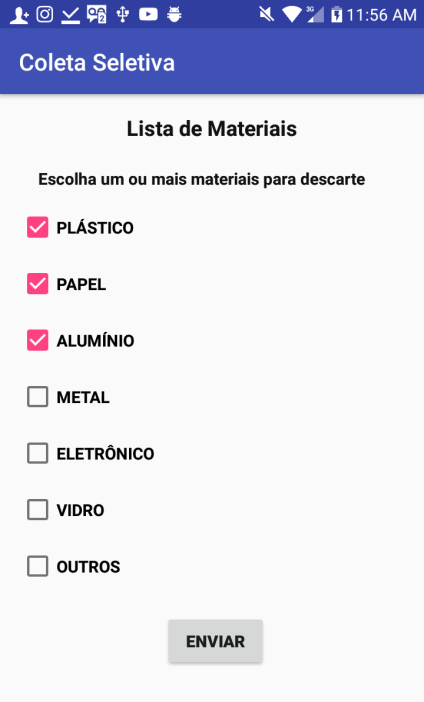
\includegraphics[width=1.93in,height=3.06in]{./media/image60.png}
	\end{Center}
	\caption{Lista de materiais}
	\label{fig:listmaterial}
\end{figure}
%%%%%%%%%%%%%%%%%%% Figure/Image No: 55 Ends here %%%%%%%%%%%%%%%%%%%%

A \autoref{fig:listmaterial} citada acima, apresenta para o usuário separador, os tipos de materiais que podem ser reciclados. Os tipos de materiais são: plástico, papel, alumínio, metal, eletrônico e vidro. Caso não tenha o tipo de material desejado na lista, o usuário poderá escolher a opção "outros". Após informar o tipo do material será possível enviar a solicitação do recolhimento do resíduo sólido.

Na \autoref{fig:local} a seguir, é apresentada a tela referente à localização do material a ser descartado pelo usuário separador. 
%%%%%%%%%%%%%%%%%%%% Figure/Image No: 56 starts here %%%%%%%%%%%%%%%%%%%%

\begin{figure}[H]
	\begin{Center}
		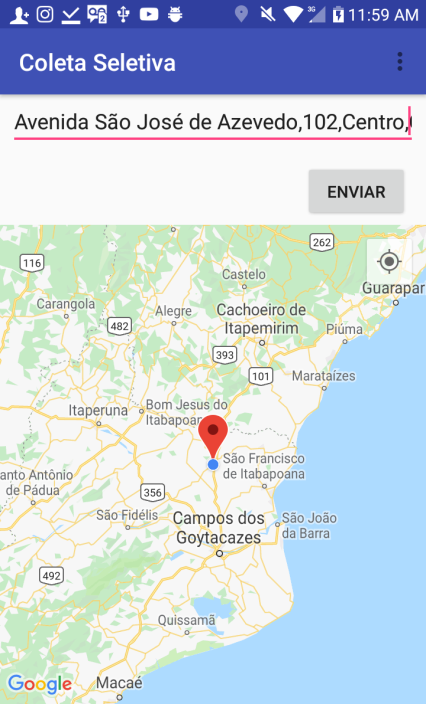
\includegraphics[width=1.93in,height=3.06in]{./media/image49.png}
	\end{Center}
	\caption{Informar localização do material}
	\label{fig:local}
\end{figure}
%%%%%%%%%%%%%%%%%%%% Figure/Image No: 56 Ends here %%%%%%%%%%%%%%%%%%%%

A \autoref{fig:local} citada acima, apresenta a tela onde o usuário separador irá informar a localização do material a ser descartado. O ponto de localização presente no mapa é referente à localização do usuário. O mapa contém opções de botões para afastar e aproximar o mapa e um controle de zoom bastante prático, apenas com o deslizar do toque na tela.

Na \autoref{fig:recolhimento} abaixo, é apresentada a lista de solicitações do recolhimento do material.
%%%%%%%%%%%%%%%%%%%% Figure/Image No: 60 starts here %%%%%%%%%%%%%%%%%%%%

\begin{figure}[H]
	\begin{Center}
		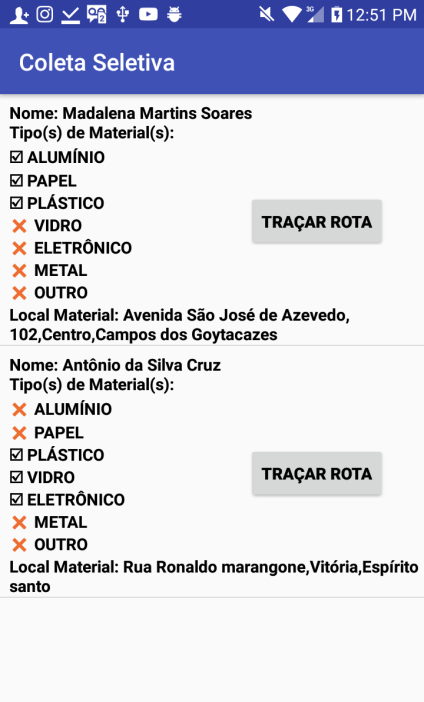
\includegraphics[width=1.93in,height=2.63in]{./media/image52.png}
	\end{Center}
	\caption{Solicitações do recolhimento do material}
	\label{fig:recolhimento}
\end{figure}

A \autoref{fig:recolhimento} citada cima, apresentada a lista com a requisições de coleta de material que serão visualizadas pelo usuário catador. Os dados apresentados nesta lista são: o nome do separador, o tipo de material e o endereço da localização deste material. Ao clicar no botão "traçar rota" o catador, será redirecionado para a tela correspondente.

Na \autoref{fig:rota} a seguir, é apresentada a tela traçar rota. 
%%%%%%%%%%%%%%%%%%%% Figure/Image No: 61 starts here %%%%%%%%%%%%%%%%%%%%

\begin{figure}[H]
	\begin{Center}
		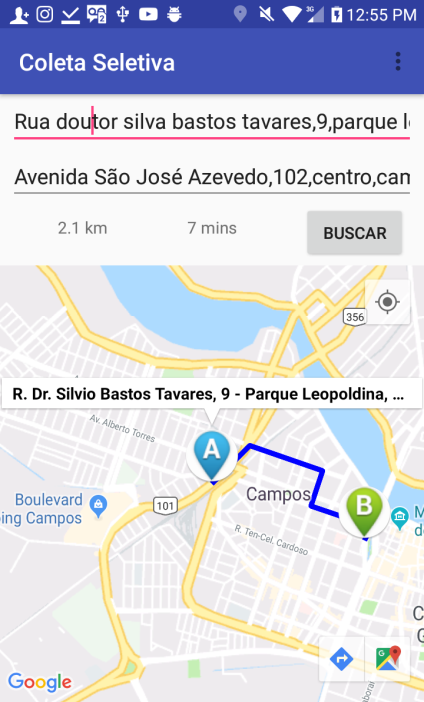
\includegraphics[width=1.92in,height=3.06in]{./media/image43.png}
	\end{Center}
	\caption{Tela traçar rota}
	\label{fig:rota}
\end{figure}
%%%%%%%%%%%%%%%%%%%% Figure/Image No: 61 Ends here %%%%%%%%%%%%%%%%%%%%

A \autoref{fig:rota}, apresentada acima, observa-se o funcionamento da rota para o recolhimento do material. O usuário de perfil catador insere a sua localização atual e o local onde o material foi depositado e ao realizar a busca, lhe é fornecido a duração e a distância da rota.

Na \autoref{fig:cadastro} a seguir, é apresentada a tela do cadastro de usuários.

\begin{figure}[H]
	\begin{Center}
		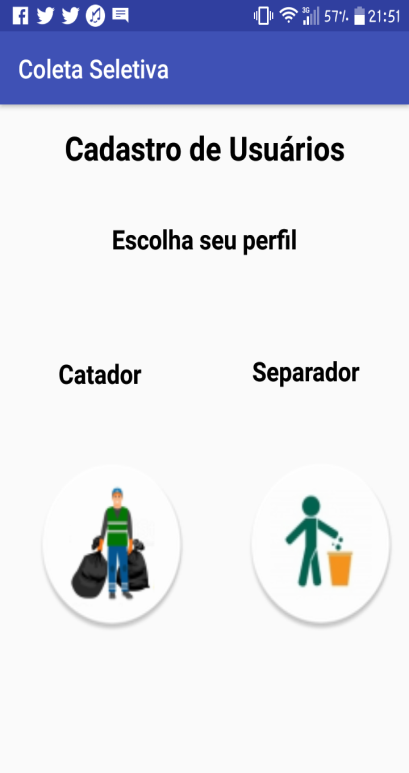
\includegraphics[width=1.92in,height=3.06in]{./media/image41.png}
	\end{Center}
	\caption{Cadastro de usuários}
	\label{fig:cadastro}
\end{figure}

O protótipo de aplicação faz uso de dois perfis: catador e separador. No ato do cadastro (\autoref{fig:cadastro}), o usuário irá escolher qual perfil se encaixa e será redirecionado para a tela correspondente. 

Na \autoref{fig:senha} a seguir, é apresentada a tela de recuperação da senha.

\begin{figure}[H]
	\begin{Center}
		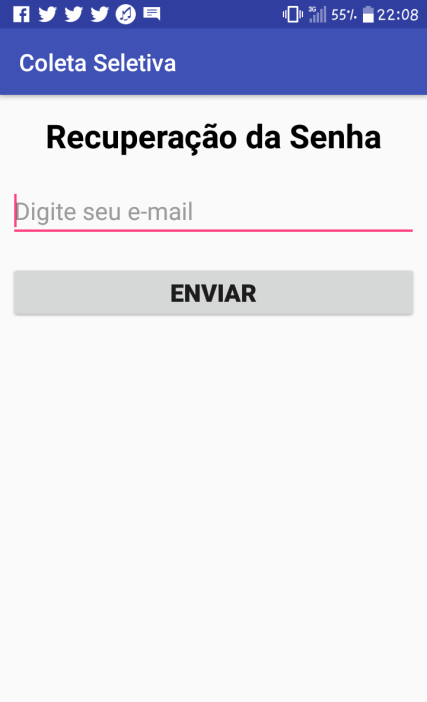
\includegraphics[width=1.92in,height=3.06in]{./media/image42.png}
	\end{Center}
	\caption{Recuperação da senha}
	\label{fig:senha}
\end{figure}

Para recuperar a senha (\autoref{fig:senha}) o usuário irá informar seu \textit{e-mail}, caso não tenha cadastro, o sistema irá informá-lo. Caso contrário, receberá um \textit{e-mail} contendo o \textit{link} e as instruções para a redefinição da senha.

Na \autoref{fig:duvida} a seguir, é apresentada a tela de tira-dúvidas.

\begin{figure}[H]
	\begin{Center}
		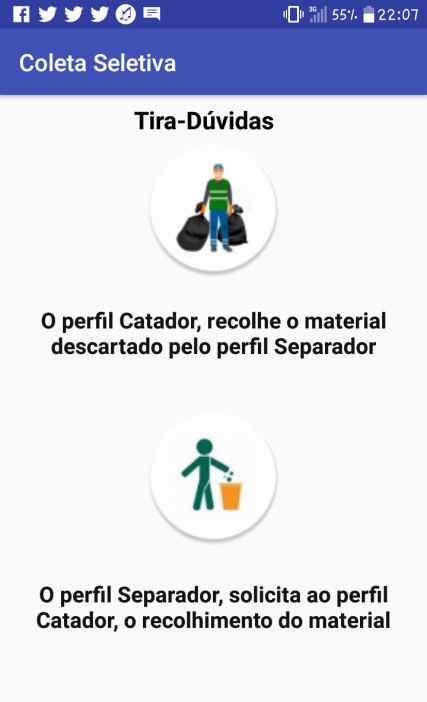
\includegraphics[width=1.92in,height=3.06in]{./media/image48.png}
	\end{Center}
	\caption{Tira-Dúvidas}
	\label{fig:duvida}
\end{figure}

A \autoref{fig:duvida} citada acima, é responsável por informar a definição dos perfis: catador e separador.

O recurso de traçar a rota contido na aplicação, permite a previsão da coleta do material, pelo fato de informar a duração e a distância até o ponto do recolhimento.

A informação do tipo de material a ser descartado pelo separador, é benéfica para o catador, pois o mesmo pode otimizar o seu tempo indo aos locais onde existem os materiais de seu interesse.

Neste Capítulo foram apresentados alguns aspectos referentes ao protótipo de aplicação implementado e aos testes realizados. Através do questionário de avaliação, foi possível confirmar que o protótipo de aplicação  foi útil e gerou interesse aos participantes do questionário.
